% SC2002 --- Chapter 4: UML Class & Sequence Diagrams (0->100 ground-up)
\chapter{UML Class \& Sequence Diagrams: Visual Contracts}
\label{ch:uml}

\begin{quote}
\emph{``A diagram is worth a thousand lines---if it has a legend.''} --- UML is not decoration; it is a precise visual contract between designer and implementer. This chapter teaches you to read and draw the two diagrams you will use most: class and sequence.
\end{quote}

\noindent\fbox{\parbox{\dimexpr\linewidth-2\fboxsep-2\fboxrule}{%
\textbf{From zero: built on Ch.~1--3.} We define UML notation from first principles---no prior modelling assumed. Class diagrams capture \emph{structure}; sequence diagrams capture \emph{behaviour over time}. Both map directly to Java.}}
\vspace{0.4em}

\section*{Learning Outcomes}
After this chapter you will be able to:
\begin{enumerate}[label=(L\arabic*)]
    \item read and draw UML class diagrams: classes, attributes, operations, visibility, associations, multiplicity, generalisation, dependency, composition/aggregation;
    \item read and draw UML sequence diagrams: lifelines, messages (sync/async/return), alt/opt/loop fragments, creation/destruction;
    \item translate a class diagram to Java skeletons and a sequence diagram to method-call order;
    \item choose the right diagram for a question (structure vs.\ interaction) and keep them consistent;
    \item critique a UML diagram for completeness, multiplicity errors, and directionality.
\end{enumerate}

% ============================================================
\section{Class Diagrams: Structure at a Glance}
\label{sec:class-diagrams}
A class diagram shows the \emph{static} structure: what types exist, what each knows, and how they relate. Notation is compact but precise.

\begin{figure}[h]
\centering
\resizebox{\linewidth}{!}{%
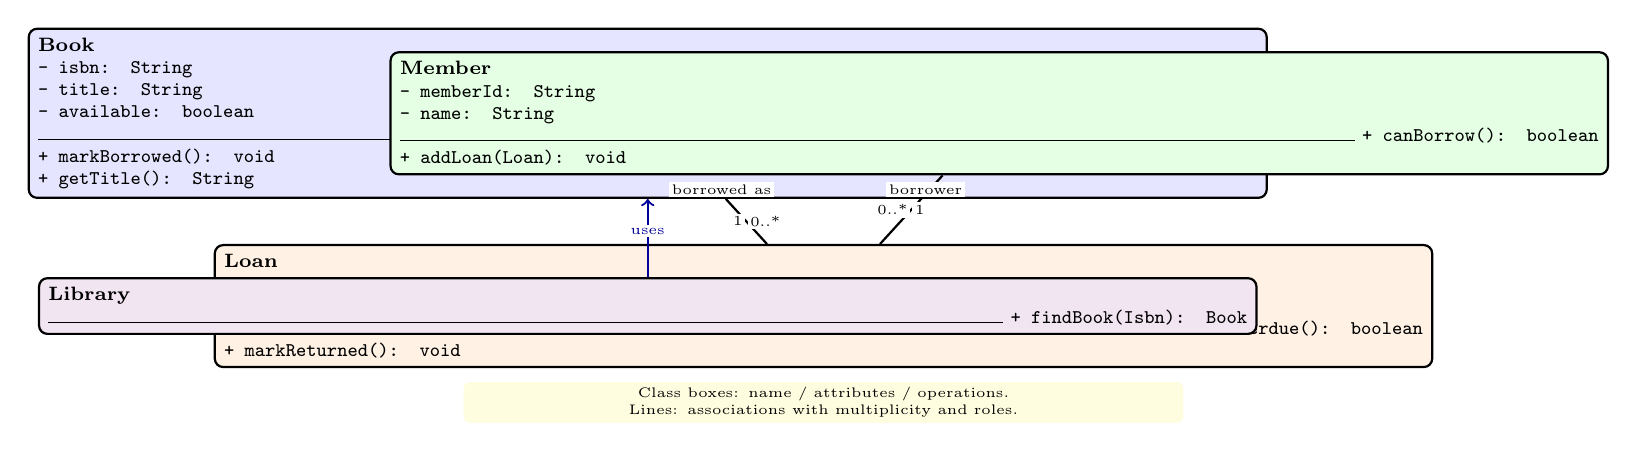
\begin{tikzpicture}[scale=0.72, every node/.style={font=\scriptsize}]
\tikzset{umlclass/.style={draw,thick,fill=blue!6,rounded corners=3pt,minimum width=3.0cm,align=left}}
\node[umlclass,fill=blue!10] (book) at (0,0) {
  \textbf{Book} \\
  \texttt{- isbn: String}\\
  \texttt{- title: String}\\
  \texttt{- available: boolean}\\ \rule{\linewidth}{0.4pt}
  \texttt{+ isAvailable(): boolean}\\
  \texttt{+ markBorrowed(): void}\\
  \texttt{+ getTitle(): String}
};
\node[umlclass,fill=green!10] (member) at (6.2,0) {
  \textbf{Member} \\
  \texttt{- memberId: String}\\
  \texttt{- name: String}\\ \rule{\linewidth}{0.4pt}
  \texttt{+ canBorrow(): boolean}\\
  \texttt{+ addLoan(Loan): void}
};
\node[umlclass,fill=orange!10] (loan) at (3.1,-3.4) {
  \textbf{Loan} \\
  \texttt{- dueDate: LocalDate}\\
  \texttt{- returned: boolean}\\ \rule{\linewidth}{0.4pt}
  \texttt{+ isOverdue(): boolean}\\
  \texttt{+ markReturned(): void}
};
\draw[thick] (book) -- (loan) node[midway,left,font=\tiny,fill=white,inner sep=1pt] {1} node[midway,right,font=\tiny,fill=white,inner sep=1pt] {0..*};
\draw[thick] (member) -- (loan) node[midway,right,font=\tiny,fill=white,inner sep=1pt] {1} node[midway,left,font=\tiny,fill=white,inner sep=1pt] {0..*};
\node[font=\tiny,fill=white,inner sep=1pt] at (1.3,-1.35) {borrowed as};
\node[font=\tiny,fill=white,inner sep=1pt] at (4.9,-1.35) {borrower};
% composition example
\node[umlclass,fill=violet!10,minimum width=2.6cm] (lib) at (0,-3.4) {
  \textbf{Library} \\ \rule{\linewidth}{0.4pt}
  \texttt{+ findBook(Isbn): Book}
};
\draw[->,thick,blue!60!black] (lib) -- (book) node[midway,above,font=\tiny,fill=white,inner sep=1pt] {uses};
\node[font=\tiny,align=center,fill=yellow!12,rounded corners=2pt,inner sep=2pt,text width=9cm] at (3.1,-5.1) {Class boxes: name / attributes / operations. Lines: associations with multiplicity and roles.};
\end{tikzpicture}%
}
\caption{Library class diagram: \texttt{Book}--\texttt{Loan}--\texttt{Member} associations with multiplicities; \texttt{Library} depends on \texttt{Book}.}
\label{fig:uml-class-library}
\end{figure}

\paragraph{Class box.} Three compartments: name (bold, abstract in \emph{italics}), attributes (\texttt{visibility name: Type}), operations (\texttt{visibility name(params): ReturnType}). Visibility: \texttt{+} public, \texttt{-} private, \texttt{\#} protected, \texttt{\textasciitilde} package.

\paragraph{Relationships.}
\begin{itemize}[itemsep=0.25em]
    \item \emph{Association} (solid line): ``knows about.'' Label with role names and \emph{multiplicity}: \texttt{1}, \texttt{0..1}, \texttt{*}, \texttt{1..*}, \texttt{0..*}.
    \item \emph{Composition} (filled diamond): part dies with whole (\texttt{Library} \texttt{1} $\blacklozenge$-- \texttt{Loan} \texttt{*}---if Library deleted, Loans deleted).
    \item \emph{Aggregation} (hollow diamond): part may outlive whole.
    \item \emph{Generalisation} (hollow triangle arrow): inheritance.
    \item \emph{Dependency} (dashed arrow): ``uses temporarily'' (parameter, local variable, static call).
\end{itemize}

\begin{lstlisting}[language=Java, caption={From class diagram to Java---multiplicity guides the collection type.}]
//  Member 1 -- 0..* Loan  => Member holds a collection of Loans
class Member {
    private String memberId;
    private List<Loan> loans = new ArrayList<>();
    public boolean canBorrow() { return loans.size() < 5; }
    public void addLoan(Loan l) { loans.add(l); }
}
class Loan {
    private Member borrower;  //  Loan * -- 1 Member
    private Book book;        //  Loan * -- 1 Book
    private LocalDate dueDate;
    public boolean isOverdue() { return LocalDate.now().isAfter(dueDate); }
}
\end{lstlisting}

% --- TikZ 2: Sequence diagram ---
\begin{figure}[h]
\centering
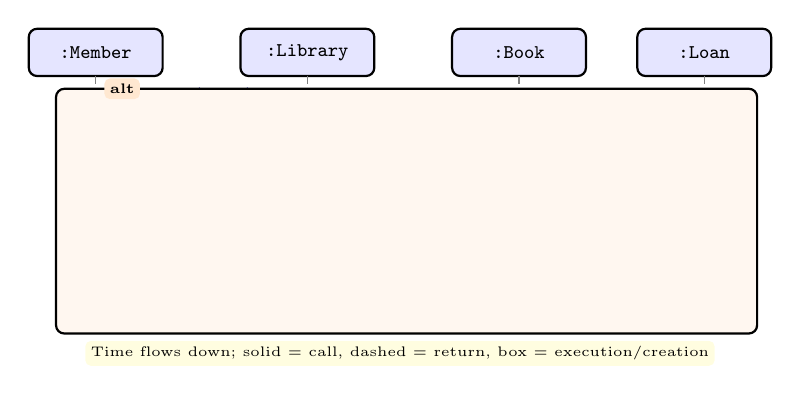
\begin{tikzpicture}[scale=0.84, every node/.style={font=\scriptsize}]
% lifelines
\foreach \x/\name in {0/Member, 3.2/Library, 6.4/Book, 9.2/Loan} {
  \node[draw,thick,fill=blue!10,rounded corners=3pt,minimum width=1.7cm,minimum height=0.6cm] at (\x,0) {\texttt{:\name}};
  \draw[dashed,gray] (\x,-0.35) -- (\x,-4.2);
}
% messages
\draw[->,thick,blue!60!black] (0,-0.85) -- (3.2,-0.85) node[midway,above,font=\tiny] {\texttt{borrow(bookId)}};
\draw[->,thick,blue!60!black] (3.2,-1.30) -- (6.4,-1.30) node[midway,above,font=\tiny] {\texttt{isAvailable()}};
\draw[->,thick,green!60!black,dashed] (6.4,-1.70) -- (3.2,-1.70) node[midway,above,font=\tiny] {\texttt{true}};
\draw[->,thick,blue!60!black] (3.2,-2.15) -- (0,-2.15) node[midway,above,font=\tiny] {\texttt{canBorrow()}};
\draw[->,thick,green!60!black,dashed] (0,-2.55) -- (3.2,-2.55) node[midway,above,font=\tiny] {\texttt{true}};
% create
\draw[->,thick,violet!70!black] (3.2,-3.00) -- (9.2,-3.00) node[midway,above,font=\tiny] {\texttt{create(member,book)}};
\fill[violet!18] (9.15,-3.05) rectangle (9.25,-3.9);
\draw[->,thick,green!60!black,dashed] (9.2,-3.90) -- (3.2,-3.90) node[midway,above,font=\tiny] {\texttt{loan}};
\node[font=\tiny,fill=yellow!12,rounded corners=2pt,inner sep=2pt] at (4.6,-4.55) {Time flows down; solid = call, dashed = return, box = execution/creation};
% alt fragment
\draw[thick,rounded corners=3pt,fill=orange!6] (-0.6,-0.55) rectangle (10.0,-4.25);
\node[font=\tiny\bfseries,fill=orange!18,rounded corners=2pt,inner sep=2pt] at (0.4,-0.55) {alt};
\end{tikzpicture}
\caption{Sequence diagram for \texttt{borrow}: \texttt{Member} $\to$ \texttt{Library} $\to$ \texttt{Book} checks, then \texttt{Loan} creation. Add \texttt{alt} for failure branches.}
\label{fig:uml-sequence-borrow}
\end{figure}

\section{Sequence Diagrams: Interaction Over Time}
\label{sec:sequence}
A sequence diagram shows \emph{how} objects collaborate for one scenario. Time flows downwards; each vertical dashed line is a \emph{lifeline}; horizontal arrows are \emph{messages}.

Message kinds: synchronous call (filled arrowhead, caller blocks), asynchronous (open arrowhead, fire-and-forget), return (dashed), creation (\texttt{create} with new lifeline), destruction (\texttt{X} at end). Fragments: \texttt{alt} (if/else), \texttt{opt} (if), \texttt{loop} (while/for), \texttt{ref} (reference another diagram).

\begin{remark}[Class vs.\ sequence---when to use which]
Use a class diagram to answer ``what types and relations exist?'' (structure). Use a sequence diagram to answer ``in what order do they interact for this use case?'' (behaviour). Keep them consistent: every message's target operation must appear in the class diagram.
\end{remark}

% --- TikZ 3: Fragments alt/loop ---
\begin{figure}[h]
\centering
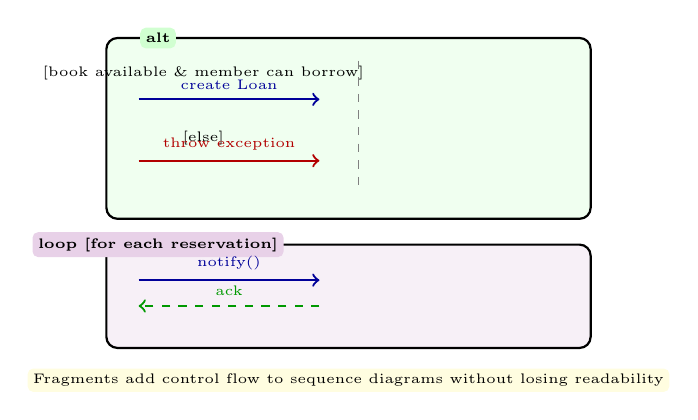
\begin{tikzpicture}[scale=0.82, every node/.style={font=\scriptsize}]
% fragment box
\draw[thick,rounded corners=4pt,fill=green!6] (-0.3,0.2) rectangle (7.2,-2.6);
\node[font=\tiny\bfseries,fill=green!18,rounded corners=2pt,inner sep=2pt] at (0.5,0.2) {alt};
\node[font=\tiny,align=left] at (1.2,-0.35) {[book available \& member can borrow]};
\draw[->,thick,blue!60!black] (0.2,-0.75) -- (3.0,-0.75) node[midway,above,font=\tiny] {create Loan};
\node[font=\tiny,align=left] at (1.2,-1.35) {[else]};
\draw[->,thick,red!70!black] (0.2,-1.70) -- (3.0,-1.70) node[midway,above,font=\tiny] {throw exception};
\draw[dashed,gray] (3.6,-0.15) -- (3.6,-2.15);
% loop fragment below
\draw[thick,rounded corners=4pt,fill=violet!6] (-0.3,-3.0) rectangle (7.2,-4.6);
\node[font=\tiny\bfseries,fill=violet!18,rounded corners=2pt,inner sep=2pt] at (0.5,-3.0) {loop [for each reservation]};
\draw[->,thick,blue!60!black] (0.2,-3.55) -- (3.0,-3.55) node[midway,above,font=\tiny] {notify()};
\draw[->,thick,green!60!black,dashed] (3.0,-3.95) -- (0.2,-3.95) node[midway,above,font=\tiny] {ack};
\node[font=\tiny,fill=yellow!12,rounded corners=2pt,inner sep=2pt] at (3.45,-5.1) {Fragments add control flow to sequence diagrams without losing readability};
\end{tikzpicture}
\caption{Fragments: \texttt{alt} for branches, \texttt{loop} for iteration (add guards in brackets).}
\label{fig:uml-fragments}
\end{figure}

\section{From Diagrams to Code and Back: Consistency}
\label{sec:uml-consistency}
UML earns its keep only if diagrams and code agree. Two consistency rules:

\paragraph{Class $\leftrightarrow$ sequence agreement.} Every lifeline in a sequence diagram must correspond to a class (or actor) in the class diagram; every message must correspond to an operation declared on the target's class. A mismatch is a defect, not a ``detail for later.''

\paragraph{Multiplicity guides implementation.} \texttt{1} $\to$ single reference, \texttt{0..1} $\to$ \texttt{Optional<T>} or nullable reference, \texttt{*} $\to$ \texttt{List<T>} or \texttt{Set<T>}. Navigability arrows tell you where the reference lives: if only \texttt{Member $\to$ Loan} is navigable, only \texttt{Member} holds a collection.

\begin{lstlisting}[language=Java, caption={Navigability decides field placement.}]
// Association  Member 1 ---- 0..* Loan  (navigable Member -> Loan only)
class Member { private List<Loan> loans = new ArrayList<>(); } // Member holds it
class Loan { /* no back-pointer to Member unless navigable the other way */ }

// If navigable both ways, both hold references (keep in sync via one owner method)
class Loan2 { private Member borrower; private Book book; }
\end{lstlisting}

\paragraph{Tooling and levelling.} Keep diagrams at the level of the audience: analysis diagrams omit private helpers; design diagrams include them. Generate class skeletons from UML (PlantUML, IntelliJ) and round-trip carefully---never let the diagram drift from the code after the first sprint.

\begin{remark}[Diagram smells]
God-class box with 30 operations, associations without multiplicity, sequence diagrams that never show \texttt{alt} for error paths, and lifelines labelled with class names instead of roles (\texttt{:Book} vs.\ \texttt{Book}) are all review flags.
\end{remark}

\subsection{Worked Consistency Check: Borrow Use Case}
Given the class diagram in Fig.~\ref{fig:uml-class-library} and the sequence in Fig.~\ref{fig:uml-sequence-borrow}, verify: (i) \texttt{Library.borrow} exists on \texttt{Library}, (ii) \texttt{Book.isAvailable} exists on \texttt{Book}, (iii) \texttt{Member.canBorrow} exists on \texttt{Member}, (iv) \texttt{Loan} creation parameters match its constructor, (v) multiplicities allow the new \texttt{Loan} (member has $<5$ loans). Any failure is a modelling defect caught before coding.

\paragraph{Review checklist for a class diagram.} Are all associations labelled with multiplicity and role? Is navigability correct (who holds the reference)? Are generalisations substitutable (LSP)? Are dependencies dashed and associations solid? For a sequence diagram: do \texttt{alt} branches cover error paths? Are lifelines created/destroyed at the right time? Do guards read as boolean expressions?

\subsection{Visual Editing Workflow}
Draw class diagrams top-down (most stable abstractions at the top, details at the bottom) and sequence diagrams left-to-right in call order. Colour by layer (blue=domain, green=service, orange=data) so a reader can see architectural boundaries at a glance. Keep a one-page legend (visibility symbols, line styles, fragment names) on the first UML page of any document.

\begin{center}
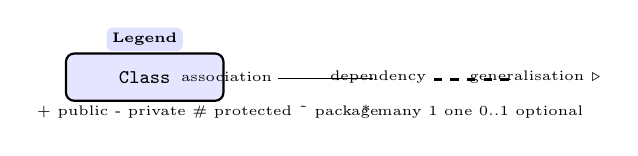
\begin{tikzpicture}[scale=0.80, every node/.style={font=\scriptsize}]
\node[font=\tiny\bfseries,fill=blue!12,rounded corners=2pt,inner sep=2pt] at (0,0.6) {Legend};
\node[draw,thick,fill=blue!10,rounded corners=3pt,minimum width=2.0cm,minimum height=0.6cm] at (0,0) {\texttt{Class}};
\node[font=\tiny] at (2.1,0) {association \rule[0.4ex]{1.2cm}{0.7pt}};
\node[font=\tiny] at (4.4,0) {dependency \tikz\draw[dashed,thick](0,0)--(1.0,0);};
\node[font=\tiny] at (6.2,0) {generalisation $\triangleright$};
\node[font=\tiny] at (1.0,-0.55) {+ public  - private  \# protected  \textasciitilde\ package};
\node[font=\tiny] at (5.2,-0.55) {* many  1 one  0..1 optional};
\end{tikzpicture}
\end{center}
A legend removes ambiguity and costs one small TikZ---always include it in hand-ins.

\section{Chapter Notes}
UML 2.5.1 is the current standard (OMG). We cover only class + sequence---the highest-ROI pair. State-machine and activity diagrams are useful complements (SC2006/advanced modelling). Tools: PlantUML, IntelliJ UML, Visual Paradigm; any tool that exports clear, colour-legended diagrams suffices.

\section{Exercises}
\label{sec:ch04-exercises}
\begin{enumerate}[label=E4.\arabic*, leftmargin=*, itemsep=0.8em]
    \item \textbf{Class diagram reading.} Given the library class diagram in Fig.~\ref{fig:uml-class-library}, list every association's multiplicity, role names, and navigability. Write the Java field declarations that realise each association.
    \item \textbf{Composition vs.\ aggregation.} Model \texttt{Order}--\texttt{OrderLine} and \texttt{Department}--\texttt{Professor}. Which should be composition and which aggregation? Justify via lifecycle (does part die with whole?).
    \item \textbf{Sequence to code.} Translate Fig.~\ref{fig:uml-sequence-borrow} into a Java \texttt{Library.borrow(memberId, bookId)} skeleton that returns a \texttt{Loan} or throws. Show where each message becomes a method call.
    \item \textbf{Fragment modelling.} Draw a sequence diagram for ``member reserves an unavailable book; when the book is returned the next reserver is notified.'' Use \texttt{alt} and \texttt{loop} fragments.
    \item \textbf{Consistency check.} A class diagram shows \texttt{Loan} with no \texttt{isOverdue()} but the sequence diagram calls it. A teammate says ``it's fine, we will add it later.'' Explain why this inconsistency is a defect and how tool or review can catch it.
\end{enumerate}
% End of Chapter 4
